% !TeX spellcheck = nl_NL
%%=============================================================================
%% Methodologie
%%=============================================================================

\chapter{\IfLanguageName{dutch}{Methodologie}{Methodology}}
\label{ch:methodologie}

%% TODO: Hoe ben je te werk gegaan? Verdeel je onderzoek in grote fasen, en
%% licht in elke fase toe welke stappen je gevolgd hebt. Verantwoord waarom je
%% op deze manier te werk gegaan bent. Je moet kunnen aantonen dat je de best
%% mogelijke manier toegepast hebt om een antwoord te vinden op de
%% onderzoeksvraag.
Om het effect van zowel K8s \textit{best-practices} als K8s beveiligings-tools op een cluster te onderzoeken werd er gekozen om het onderzoek in 3 scenario's onder te verdelen. Met als doel gegevens te verzamelen over enkele criteria, namelijk het resource gebruik, de stabiliteit en de opstarttijd van de cluster. Voordat we aan de scenario's kunnen beginnen, worden eerst nog alle stappen doorlopen voor het opzetten van de cluster. Nadat de cluster opgezet is zullen we beginnen met het eerste scenario, namelijk het opzetten van een basis cluster om de functionaliteit van K8s aan te tonen en om baseline gegevens te verzamelen voor het onderzoek. Deze cluster zal dienen als basis om verdere scenario's verder uit te werken. Als tweede worden er enkele ``best-practice'' gehanteerd bij het opzetten en de configuratie van de cluster, dit om te onderzoeken wat voor effect deze hebben op de cluster. Ten slotte zal er bij het opzetten en configureren van de cluster gebruik gemaakt worden van enkele K8s beveiligings-tools, dit om te testen wat deze precies doen en wat voor effect deze kunnen hebben op de criteria. 

Gedurende dit onderzoek werd er gebruik gemaakt van de volgende hardware en software:

\begin{itemize}
	\item Besturingssysteem: Pop!\_OS 20.10 x86\_64
	\item Host systeem: MSI GL62 7REX
	\item Kernel: 5.11.0-7614-generic (Linux)
	\item Cloud provider: Linode\footnote{cloud.linode.com/}
	\item Nodes: 3 X Linode 2GB (1CPU core, 2GB RAM, 50GB opslag, Debian 5.10.24-1)
\end{itemize}

\section{Opzetten van de Kubernetes cluster}
In dit hoofdstuk zal de basis cluster opgezet worden. Deze manier van werken zal ook gebruikt worden om de andere scenario's uit te voeren.

Voor het opzetten van de cluster zijn er maar drie onderdelen nodig. 
\begin{itemize}
	\item Account bij een cloud provider, in dit geval Linode.
	\item Kubectl om de cluster te besturen.
	\item De Docker image om een applicatie te deployen op de cluster.
\end{itemize}

Aangezien Kubectl op zowel Linux, Windows als MacOS kan draaien, en de cluster zelf bij de cloud provider wordt gehost kunnen deze scenario's op bijna elke computer worden nagebootst. De stappen in volgende hoofdstukken worden allemaal uitgevoerd op een Linux systeem en kunnen dus verschillen op Windows of MacOS. Het is ook aangeraden om een nieuwe directory aan te maken zodat alle bestanden op eenzelfde plaats te vinden zijn.

Voor dit onderzoek zal gebruik gemaakt worden van de ingebouwde ``Linode Kubernetes Engine''(LKE). Deze installeert automatisch de correcte onderdelen op de verschillende worker nodes en creëert ook een gratis master node. Hiervoor werd gekozen omdat het volledig opzetten van een K8s cluster niet binnen de scope van dit onderzoek ligt. Door gebruik te maken van de LKE kunnen we ons dus focussen op de beveiliging van de cluster. 

\subsection{Linode Kubernetes cluster}
Hieronder worden de verschillende stappen die doorlopen zijn bij het opzetten van een Linode K8s cluster beschreven.

Voor het creëren van een cluster in Linode hebben we enkel een Linode account nodig. Het aanmaken van de cluster zelf is zeer gemakkelijk en gebeurt via cloud.linode.com > Kubernetes > Create Cluster. Vul dan de naam, regio en versie van de cluster in zoals in figuur \ref{fig:LinodeNaam}.

\begin{figure}[h]
	\centering
	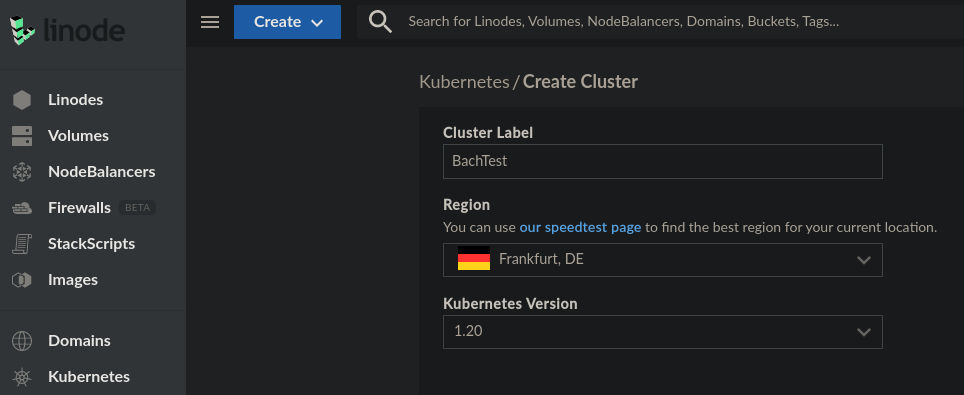
\includegraphics[width=\linewidth]{img/LinodeClusterNaam.png}
	\caption{Aanmaken Linode cluster}
	\label{fig:LinodeNaam}
\end{figure}

Vervolgens kunnen we nodes toevoegen aan de cluster. Voor dit onderzoek gaan we een kleinschalige cluster opzetten met drie worker nodes en één master node. In figuur \ref{fig:LinodeAddNodes} zijn de verschillende soorten nodes die we kunnen toevoegen opgelijst. Tijdens deze scenario's zal gebruik gemaakt worden van drie ``Linode 2GB'' nodes. Daarnaast is het ook mogelijk om nodes van verschillende grotes in dezelfde cluster toe te voegen. De master node is niet meegerekend in deze drie nodes maar word door Linode gratis aangeboden bij het opzetten van een K8s cluster.

\begin{figure}[h]
	\centering
	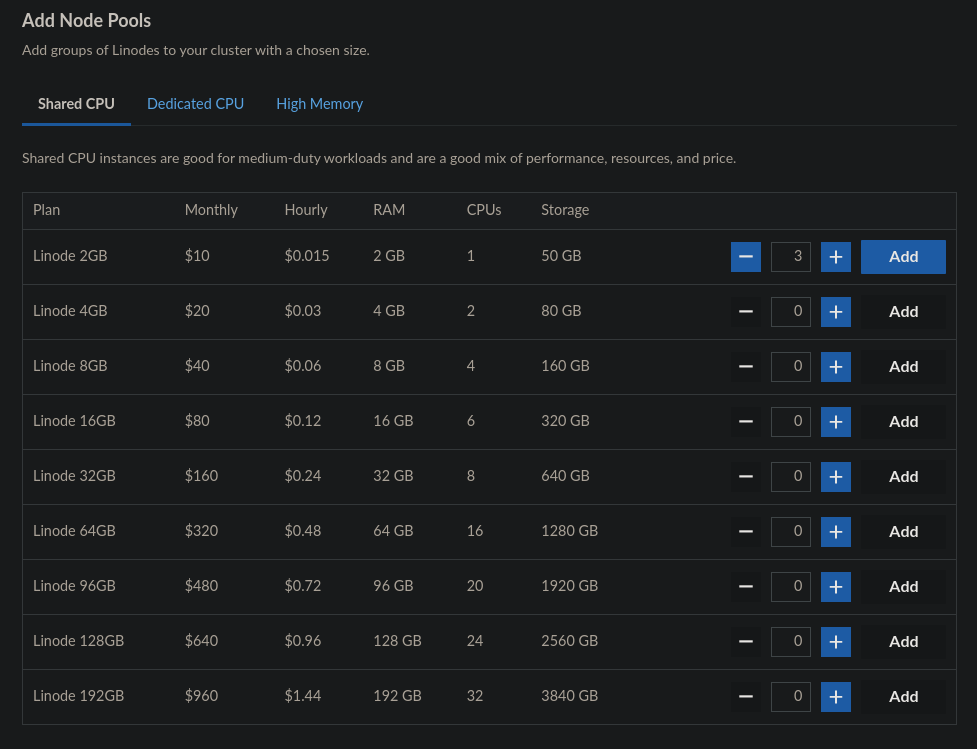
\includegraphics[width=\linewidth]{img/LinodeAddNodes.png}
	\caption{Toevoegen van nodes aan cluster}
	\label{fig:LinodeAddNodes}
\end{figure}

Als alle nodes zijn toegevoegd wordt de cluster aangemaakt. Linode zal hierbij in de achtergrond de gekozen nodes aanmaken alsook de master node klaarmaken voor gebruik. 

Eenmaal de cluster is aangemaakt en opgestart is moeten we deze nog configureren. Deze configuratie gebeurt via Kubectl in volgende stappen.

Als eerste moeten we het kubeconfig.yaml bestand downloaden van Linode. In dit bestand staan alle nodig details om te Kubectl te connecteren met onze cluster. De kubeconfig van de net aangemaakte cluster is te zien in figuur \ref{kubeconfig} (enkele waarden werden ingekort om de leesbaarheid te vergroten).

\begin{figure}[h] 
	\inputminted[fontsize=\footnotesize,linenos]{yaml}{files/BachTest-kubeconfig.yaml}
	\caption{kubeconfig.yaml}
	\label{kubeconfig}
\end{figure}

Vervolgens moet het pad naar het bestand geëxporteerd worden naar de omgevingsvariabele ``KUBECONFIG'' met het volgende commando:
\begin{minted}{bash}
$ export KUBECONFIG=<pad naar file>/kubeconfig.yaml
\end{minted}

We kunnen testen of dit gelukt is door het volgende commando uit te voeren. Dit zou de drie aangemaakte nodes in onze cluster moeten teruggeven.
\begin{minted}{bash}
$ kubectl get nodes
NAME                          STATUS   ROLES    AGE    VERSION
lke25332-32960-608682818f2e   Ready    <none>   6d4h   v1.20.5
lke25332-32960-60868281f030   Ready    <none>   6d4h   v1.20.5
lke25332-32960-608682824efd   Ready    <none>   6d4h   v1.20.5
\end{minted}

Nu Kubectl in contact staat met de ``kube-apiserver'' dewelke op de master node draait, kunnen we beginnen met het configureren van onze cluster. Dit kan zowel met ``ad-hoc'' commando's als met zogenaamde deployments die werken via het \textit{principle of desired state}. Met andere woorden specificeren de deployments de verschillende  aspecten van de cluster waarbij K8s ervoor zorgt dat aan deze specificaties voldaan worden.

Een deployment is eigenlijk niets anders dan een YAML bestand waarin beschreven wordt hoe de cluster er moet gaan uitzien. Via het volgende commando wordt een deployment op een cluster gezet.
\begin{minted}{bash}
$ kubectl apply -f deployment.yaml
\end{minted}

\subsection{Resetten van cluster}
Na het uitvoeren van elk scenario zal de cluster weer worden gereset zodat het vorige scenario geen impact kan hebben op de rest van het onderzoek. Het resetten van de cluster bestaat vooral uit het verwijderen van deployments en services. Het verwijderen van een deployment wordt gedaan aan de hand van volgend commando.
\begin{minted}{bash}
$ kubectl delete deployment <Deployment naam>
\end{minted}
Het verwijderen van een service verloopt op dezelfde manier.
\begin{minted}{bash}
$ kubectl delete service <Service naam>
\end{minted}
	
\subsection{Gegevens- verzameling en verwerking} \label{ch:gegevens}
Om conclusies te kunnen trekken uit dit onderzoek hebben we gegevens nodig. Meer bepaald gegevens over de bovengenoemde criteria, namelijk het \textit{resource} gebruik, de stabiliteit en de opstarttijd van de cluster. Deze gegevens zullen gebruikt worden om de onderzoeksvraag ``Welke impact hebben \textit{best practices} en beveiligings-tools op de criteria?'' te beantwoorden. De verzameling van deze gegevens zal gebeuren via \textit{sysstat}\footnote{github.com/sysstat/sysstat}. Dit is open source tool die ons in staat stelt om een hele hoop verschillende soorten data van ons systeem te exporteren naar bruikbare formaten (zoals JSON, CSV en XML). Deze bestanden zullen later in RStudio als bron gebruikt worden om statische modellen mee te maken. Sysstat zal op een van de Nodes in de cluster worden geïnstalleerd. Dit door middel van een ssh verbinding op te zetten met één van de Nodes en dan volgend commando uit te voeren. 
\begin{minted}{bash} 
$ sudo apt-get install sysstat
\end{minted}

Vervolgens moeten we de data collectie aanzetten door in het bestand \verb|/etc/default/sysstat| de variabele \verb|ENABLED| van\textit{''false''} naar \textit{''true''} om te zetten. Vanaf nu zal een van de meegeleverde tools, namelijk sar, elke 10 minuten een nieuwe entry maken in het bestand \verb|/var/log/sysstat/sa<dag van de maand>|. We kunnen deze bestanden uitlezen met behulp van het \verb|sar| commando. Om het CPU gebruik van het systeem om te zetten naar een csv bestand, het het later in RStudio te verwerken, kunnen we het volgende commando gebruiken. In figuur \ref{fig:CPUDataPreview} is het net gecreëerde csv bestand te zien.

\begin{minted}{bash} 
$ sar -f /var/log/sysstat/sa08 >> /root/CpuGebruikDag8.csv
\end{minted}

\begin{figure}[h]
	\centering
	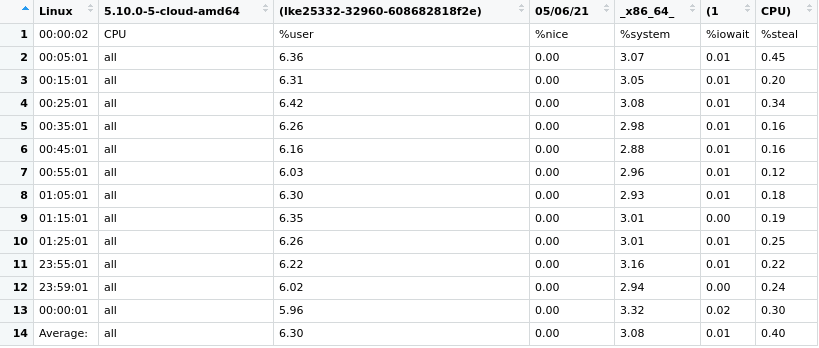
\includegraphics[width=\linewidth]{img/CPUDataPreview.png}
	\caption{Klein deel van het gebruikte csv bestand}
	\label{fig:CPUDataPreview}
\end{figure}

Vervolgens kunnen we door andere \textit{flags} mee te geven aan het sar commando verschillende soorten data uit de logbestanden halen. Het RAM gebruik kan bijvoorbeeld met volgend commando in een csv bestand worden opgeslagen.

\begin{minted}{bash} 
$ sar -f /var/log/sysstat/sa08 -r >> /root/RAMGebruikDag8.csv
\end{minted}

Als laatste moeten de gegevens lokaal op de computer beschikbaar zijn. Dit wordt gedaan door een SFTP verbinding te maken met de node waar sysstat op geïnstalleerd is en de volgende commando's uit te voeren. 

\begin{minted}{bash} 
$ sftp root@172.105.86.96
root@172.105.86.96 s password:
Connected to 172.105.86.96.
sftp> lcd /home/nick/Desktop
sftp> get CpuGebruikDag8.csv
Fetching /root/CpuGebruikDag8.csv to CpuGebruikDag8.csv
\end{minted}

Nu alle nodige gegevens zijn verzamelt kan er begonnen worden aan het verwerken van deze gegevens. Dit wordt gedaan door gebruik te maken van R en Rstudio. 

Het eerste criteria is het vergelijken van het gemiddeld resource gebruik van zowel de CPU als het RAM geheugen. Voor het CPU gebruik kan dit simpelweg door de laatste rij van het csv bestand af te lezen. Het gemiddeld gebruik van het RAM geheugen wordt niet automatisch gegenereerd door sar en moet nog berekent worden. De R code om dit te doen wordt beschreven in figuur \ref{RAMAVG}.

\begin{figure}[h] 
	\inputminted[fontsize=\footnotesize,linenos]{R}{files/dataRAMAVG.R}
	\caption{R code om boxplot van CPU gegevens te bekomen}
	\label{RAMAVG}
\end{figure}
%

Het tweede criteria is de stabiliteit van het systeem. Dit zal onderzocht worden door een Boxplot te maken op basis van de verzamelde gegevens om de hoeveelheid outliers visueel voor te stellen. De R code om dit te doen voor het CPU gebruik staat in figuur \ref{CPUBox}. In dit R script wordt het csv bestand eerst ingelezen zonder de eerste rij omdat deze niet nuttig is voor het verdere onderzoek. Vervolgens nemen we enkel de achtste kolom over omdat hier de hoeveelheid ongebruikte CPU kracht staat. Deze wordt dan afgetrokken van honderd om zo tot de gebruikte hoeveelheid CPU te komen. Als laatste wordt de naam van kolom veranderd zodat het gemakkelijker is om deze te gebruiken bij het maken van de boxplot. De laatste lijnen van het script zijn verantwoordelijk voor het creëren en opmaken van de boxplot.
%Een voorbeeld van de bekomen boxplot is te zien in figuur \ref{fig:CPUBoxEx}.

\begin{figure}[h] 
	\inputminted[fontsize=\footnotesize,linenos]{R}{files/dataCpuBox.R}
	\caption{R code om boxplot van CPU gegevens te bekomen}
	\label{CPUBox}
\end{figure}
%
%\begin{figure}[h]
%	\centering
%	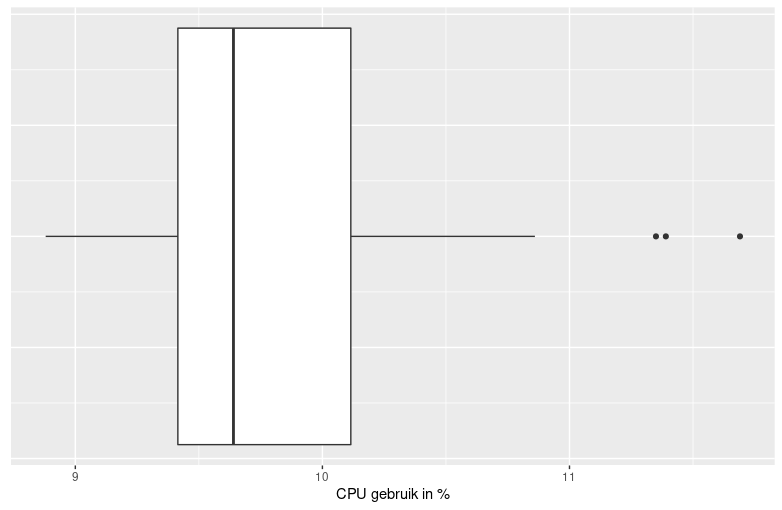
\includegraphics[width=\linewidth]{img/CPUBoxEx.png}
%	\caption{Voorbeeld boxplot CPU data}
%	\label{fig:CPUBoxEx}
%\end{figure}

Voor de gegevens van het RAM gebruik wordt op dezelfde manier te werk gegaan. De R code om de gegevens met betrekking tot het RAM geheugen wordt beschreven in figuur \ref{RAMBox}.
\begin{figure}[h] 
	\inputminted[fontsize=\footnotesize,linenos]{R}{files/dataRAMBox.R}
	\caption{R code om boxplot van CPU gegevens te bekomen}
	\label{RAMBox}
\end{figure}

Om ervoor te zorgen dat we de stabiliteit van de verschillende scenario's  met elkaar kunnen vergelijken is het ook nodig om te weten hoeveel \textit{outliers} er precies aanwezig zijn. Dit is niet altijd zo gemakkelijk te tellen als deze kort bij elkaar liggen. De \textit{outliers} kunnen allemaal opgelijst worden met het volgend commando.
\begin{minted}{bash} 
> boxplot(ram)$out
[1] 60.90 60.96 61.01 61.07 61.06 61.16 61.20 61.21 61.31 61.29 61.35
[12] 61.49 61.44 61.49 61.55 61.59 61.68 61.72 61.78 61.76 61.80 61.84
[23] 61.95 61.95 61.99 62.04 62.13 62.17 62.30 62.43 62.39 62.43 62.47
\end{minted}

Als derde criteria zal er gekeken worden naar het algemene resource gebruik van de cluster. Deze zal voorgesteld worden als een lijngrafiek waarin het resource gebruik van zowel de CPU als het RAM geheugen worden voorgesteld ten opzichte van de tijd. Het R script om dit te bekomen staat in figuur \ref{CPUGraph}. 
%Een voorbeeld van een bekomen grafiek is te zien in figuur \ref{fig:CPUgraphEx}
\begin{figure}[h] 
	\inputminted[fontsize=\footnotesize,linenos]{R}{files/dataCpuGraph.R}
	\caption{R code om grafiek van CPU gegevens te bekomen}
	\label{CPUGraph}
\end{figure}

%\begin{figure}[h]
%	\centering
%	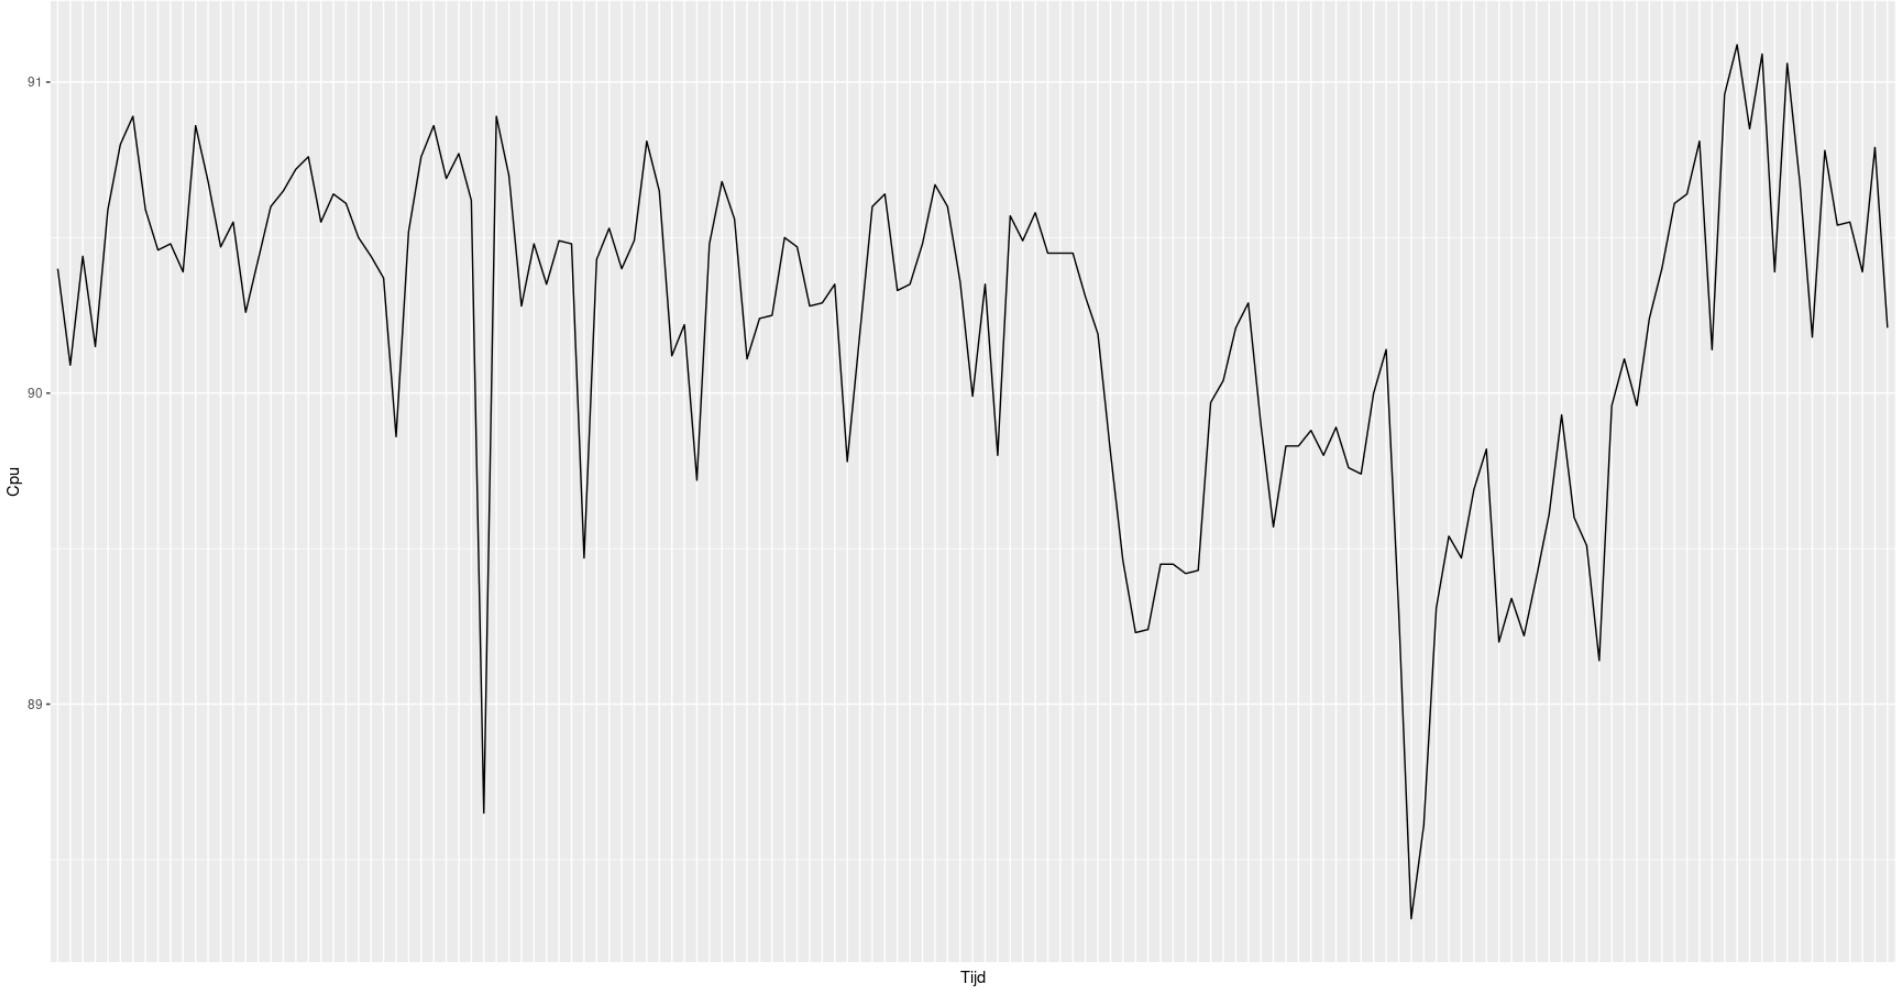
\includegraphics[width=\linewidth]{img/CPUGraphEx.png}
%	\caption{Voorbeeld grafiek CPU data}
%	\label{fig:CPUgraphEx}
%\end{figure}
Als laatste criteria zal de tijd die de node nodig heeft om op te starten vergeleken worden. Dit kan simpelweg door het volgende commando uit te voeren op de node.
\begin{minted}{bash} 
$ systemd-analyze
\end{minted}

\clearpage
\section{Scenario 1: Cluster opstelling zonder oog voor security}
%\begin{itemize}
%	\item Basic deployment van een statische website uitleggen aan de hand van commando's, screenshots en config files. 
%	\item deployment YAML tonen en deels uitleggen
%	\item Service YAML tonen en deels uitleggen
%	\item Nodige gegevens uit de cluster halen met sysstat
%	\item Verzamelde gegevens verwerken met RStudio en grafieken/statistieken tonen en uitleggen.
%\end{itemize}

%Het eerste scenario bestaat eruit om een simpele cluster op te zetten zonder specifiek oog te hebben voor de beveiliging. De deployment die zal gebruikt worden wordt in figuur \ref{basicDeploy} weergegeven. Hierin wordt een simpele demo website opgezet door gebruik te maken van de image \verb|thenetworkchuck/nccoffee:pourover|. Het aantal pods dat wordt gecreëerd wordt bepaald door de waarde van de \verb| replicas| variabele, in dit geval worden er 3 pods gecreëerd. Er wordt aangeraden om in een productieomgeving het aantal pods en nodes ongeveer gelijk te houden. De variabele \verb|imagePullPolicy: Always| zorgt ervoor dat de Docker image telkens moet worden gedownload van de registry, ook al is deze locaal aanwezig. 
Het eerste scenario bestaat eruit om een simpele cluster op te zetten zonder specifiek oog te hebben voor de beveiliging. De deployment die zal gebruikt worden wordt in figuur \ref{basicDeploy} weergegeven. Enkele van de variabelen worden hieronder uitgelegt: 
\begin{itemize}
	\item \verb|image: thenetworkchuck/nccoffee:pourover|: Dit is de Docker image met de statische demo site.
	\item \verb|replicas:3|: Het aantal pods die moeten worden gecreëerd wordt door deze variabele ingesteld. In dit geval zijn dat er 3.
	\item \verb|imagePullPolicy: Always|: Deze variabele zorgt er in dit scenario voor dat de Docker image steeds word gedownload uit de registry als de deployment wordt gebruikt.
	\item \verb|containerPort: 80|: Dit zorgt ervoor dat de site via poort 80 beschikbaar zal zijn.
\end{itemize}

\begin{figure}[h] 
	\centering
	\inputminted[fontsize=\footnotesize,linenos]{yaml}{files/deployment.yaml}
	\caption{deployment.yaml}
	\label{basicDeploy}
\end{figure}

Als de deployment YAML bestand klaar is kan deze met volgend commando op de cluster zetten.
\begin{minted}{bash} 
$ kubectl apply -f deployment.yaml
\end{minted}
Het opzetten van de pods kan gevolgt worden met het volgende commando. In figuur \ref{fig:getPodsDeployment1} is te zien hoe de pods een voor een klaargemaakt worden.
\begin{minted}{bash} 
$ kubectl get pods
\end{minted}

\begin{figure}[h]
	\centering
	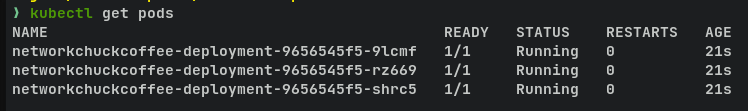
\includegraphics[width=\linewidth]{img/kubectlGetPodsDeployment1.png}
	\caption{Pods worden klaargemaakt}
	\label{fig:getPodsDeployment1}
\end{figure}

Als we nu de deployment willen aanpassen zonder de cluster volledig af te breken kunnen we het commando 
\begin{minted}{bash} 
$ kubectl edit deployments networkchuckcoffee-deployment
\end{minted}
gebruiken. In figuur \ref{editDeploy1} is de output van dit commando te zien. Als we in dit bestand bijvoorbeeld de \verb|replicas| variabele zouden aanpassen en het bestand opstaan, zal K8s merken dat er iets is veranderd. Omdat er gebruik wordt gemaakt van het ``Principle of desired state'' zal er automatisch aan de nieuwe specificaties worden voldaan. Om dit aan te tonen zal de variabele veranderd worden van drie naar vijf.

%\begin{figure}[ht]
%	\centering
%	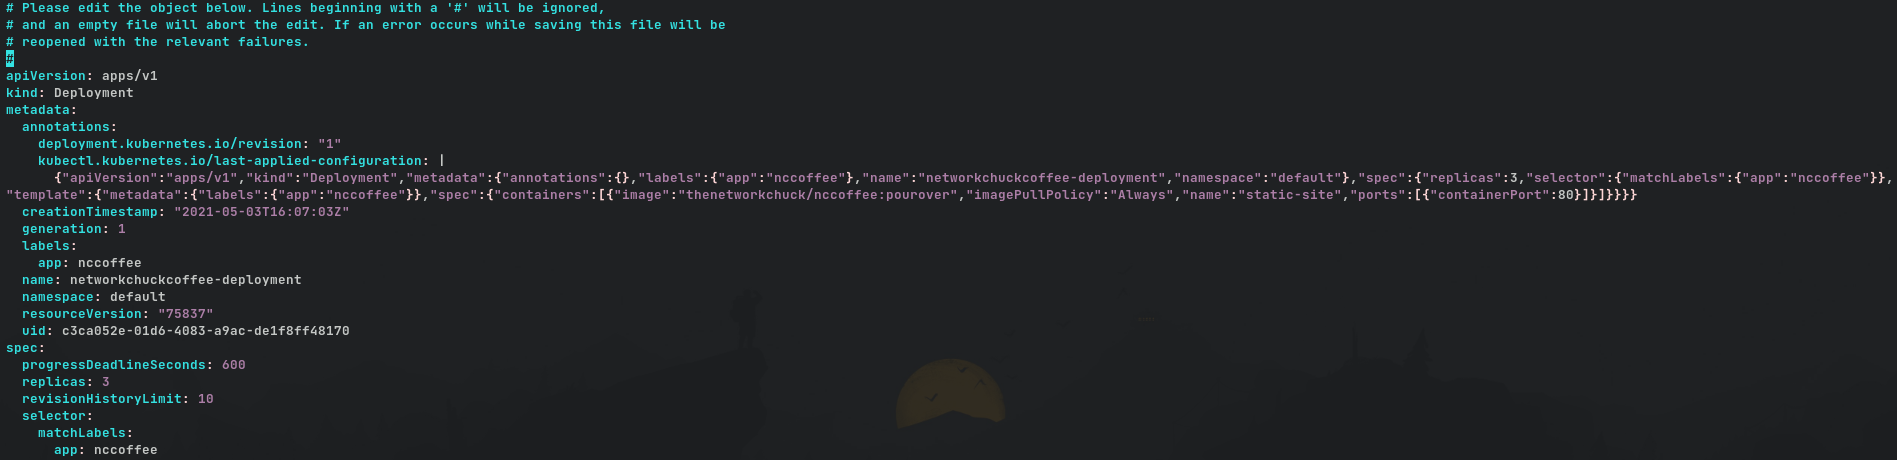
\includegraphics[width=\linewidth]{img/editDeployment1.png}
%	\caption{Output ``kubectl edit deployments'' commando}
%	\label{fig:editDeployment1}
%\end{figure}

\begin{figure}[h] 
	\inputminted[fontsize=\footnotesize,linenos]{yaml}{files/editDeployment.yaml}
	\caption{Output ``kubectl edit deployment'' commando}
	\label{editDeploy1}
\end{figure}

Als we het aantal replicas verhoogd hebben van drie naar 5 en het \verb|kubectl get pods| commando uitvoeren krijgen we, zoals in figuur \ref{fig:kubectlGetPodsEditDeploy1} te zien, dat er twee extra pods worden bijgemaakt. Deze pods worden via de \textit{scheduler} op de master node verdeeld over de drie nodes in onze cluster.
\begin{figure}[h]
	\centering
	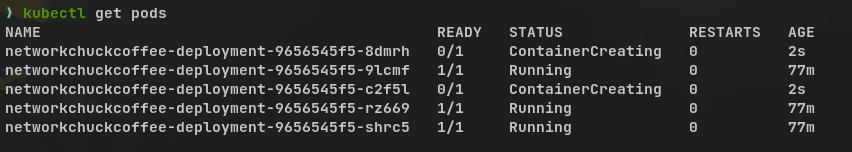
\includegraphics[width=\linewidth]{img/kubectlGetPodsEditDeploy1.png}
	\caption{Pods worden klaargemaakt}
	\label{fig:kubectlGetPodsEditDeploy1}
\end{figure}

Nu we klaar zijn met het opzetten van de deployment is het mogelijk om de cluster bloot te stellen aan het internet. Momenteel is het nog niet mogelijk om de site van buiten de cluster te bekijken. Dit komt omdat er nog geen ``service'' draait die de cluster openzet naar het internet. De service die hier zal opgezet worden zal een ``loadbalancer'' creëren op Linode die automatisch al het verkeer verdeeld over alle pods in de cluster. Het YAML bestand om de service aan te maken is te zien in figuur \ref{service1}. De code \verb|selector:app: nccoffee| zorgt ervoor dat de loadbalancer het verkeer tussen alle pods waar de applicatie ``nccoffee'' op draait verdeelt. Wanneer er pods bijkomen of verdwijnen zal de loadbalancer zich automatisch aanpassen. 

\begin{figure}[h] 
	\inputminted[fontsize=\footnotesize,linenos]{yaml}{files/testservice.yaml}
	\caption{service.yaml}
	\label{service1}
\end{figure}



Het volgend commando kan gebruikt worden om het publieke IP-adres van de loadbalancer te vinden. 
\begin{minted}{bash} 
$ kubectl get services
\end{minted}

Er is ook een manier om een meer gedetailleerde beschrijving van de service te krijgen. Namelijk door middel van het volgend commando. In figuur is de output van dit commando en alle informatie over de loadbalancer service te zien. De IP-adressen die worden getoond bij \verb|Endpoints:| zijn de IP-adressen van alle achterliggende pods waar de ``nccoffee'' applicatie op draait. Als er nu naar het publieke IP-adres van de loadbalancer wordt gesurft is de demo website te zien zoals in figuur \ref{fig:demoSite1}.
\begin{minted}{bash} 
$ kubectl describe services coffee-service 
\end{minted}

\begin{figure}[h]
	\centering
	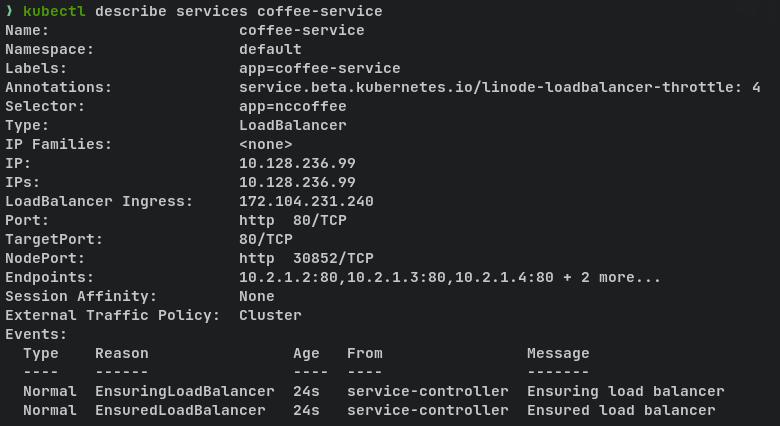
\includegraphics[width=\linewidth]{img/kubectlDescriveService1.png}
	\caption{Informatie over de loadbalancer service.}
	\label{fig:kubectlDescriveService1}
\end{figure}

\begin{figure}[h]
	\centering
	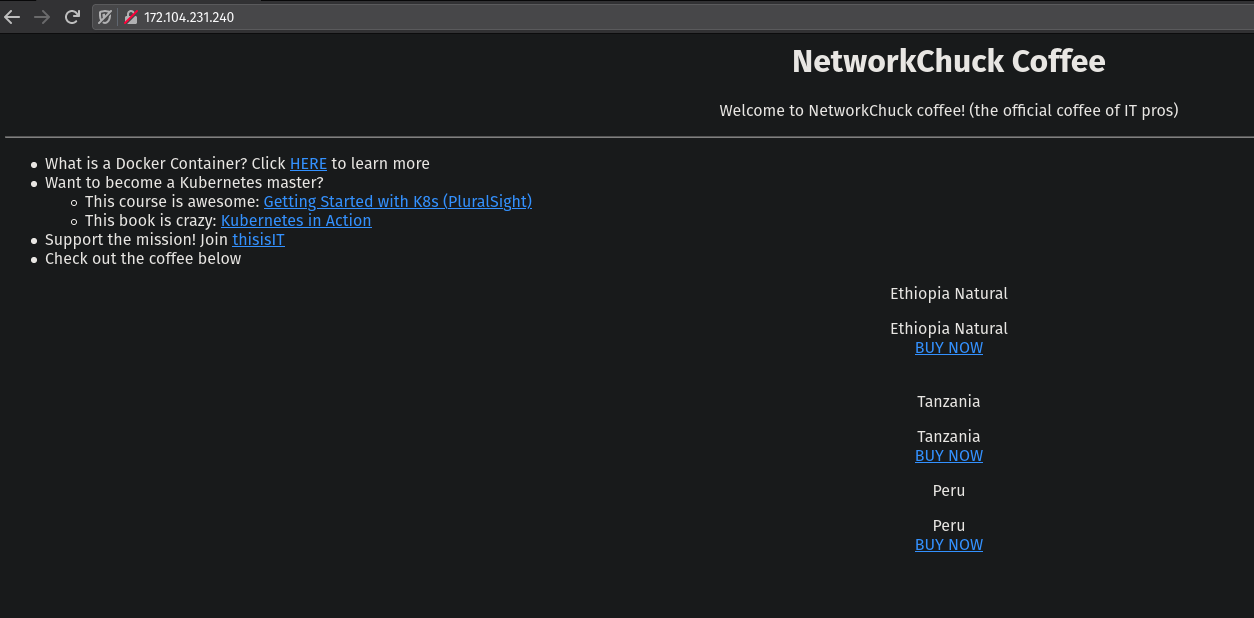
\includegraphics[width=\linewidth]{img/demoSite1.png}
	\caption{De demo website is nu zichtbaar vanop het internet.}
	\label{fig:demoSite1}
\end{figure}

\clearpage
\section{Scenario 2: Cluster opstelling met gebruik van best practices}
Het tweede scenario bestaat eruit om een simpele cluster op te zetten en gebruik te maken van enkele \textit{security best practices}. \textit{Best-practices} zoals het gebruik maken van een \textit{trusted base image} en een \textit{privite registry} zullen niet gebruikt worden omdat deze vooral dienen om de ontwikkeling van een container applicatie te beveiligen. \textit{Pod Security Policies} en \textit{RBAC} zullen wel toegepast worden op de cluster. 

Als eerste zullen er enkele Security Policies geconfigureerd worden. Het ``PodSecurityPolicy.YAML'' bestand is te zien in figuur \ref{securePol}, enkele van de variabelen worden hieronder uitgelegd: 

%https://kubernetes.io/docs/concepts/policy/pod-security-policy/

\textbf{seccomp.security.alpha.kubernetes.io/defaultProfileName:'runtime/default'}: Op Linode worden nodes automatisch vooraf geinstalleerd en geconfigureerd met AppArmor (gelijkaardig aan SELinux). Deze variabele zorgt ervoor dat de standaard ``container runtime'' profiel wordt gebruikt. Nog een mogelijke optie is \textit{Docker runtime engine}(in dit geval werd deze al standaard ingesteld).

\textbf{privileged: false} beslist of er geprivilegieerde pods aangemaakt kunnen worden. Dit staat standaard op ``false'' en moet enkel op ``true'' gezet worden wanneer een pod andere onderdelen van host nodig heeft om te werken. 

\textbf{allowPrivilegeEscalation: false}: Dit zorgt ervoor dat de user ID niet kan veranderd worden. Een ``child-process'' kan hierdoor dus ook nooit meer privileges krijgen dan de ``Parent-process''. Door deze boolean op ``false'' te zetten wordt het moeilijker voor een aanvaller om aan ``privilege escalation'' te doen.

\textbf{hostNetwork: false}: Deze variabele geeft een pod de mogelijkheid om het netwerk van de host te gebruiken. Zo kan deze ook applicaties, die de via de \textit{localhost} werken, zien en deze aanpassen. Het wordt hier op ``false'' gezet omdat deze functie niet nodig is.

\textbf{runAsUser: MustRunAsNonRoot}: Hier wordt de user ID gecontroleerd waarmee de Pods worden aangemaakt. De waarde ``MustRunAsNonRoot'' zorgt ervoor dat de containers niet door de root gebruiker kunnen worden aangemaakt. Dit wordt vooral gebruikt om te voorkomen dat iemand die (ongewenst) root privileges heeft verkregen nieuwe (onveilige) containers kan creëren.

\textbf{SupplementalGroups: 'MustRunAs'} verplicht hier het gebruik van een ``non-root'' groep bij het aanmaken van nieuwe pods. 

\textbf{ReadOnlyRootFilesystem: false} laat het aanmaken van containers met een aanpasbare ``root filesystem'' toe. Door deze variabele op ``true'' te zetten zou elke nieuwe container aangemaakt worden met een ``Read-only root filesystem''.

\begin{figure}[h] 
	\centering
	\inputminted[fontsize=\footnotesize,linenos]{yaml}{files/securePol.yaml}
	\caption{securePol.yaml}
	\label{securePol}
\end{figure}

Nadat de PodSecurityPolicy is opgesteld kan deze met volgend commando op de cluster toegepast worden.
\begin{minted}{bash} 
$ kubectl create -f securePol.yaml
\end{minted}

De PodSecurityPolicies die op de cluster actief zijn kunnen met volgend commando opgevraagd worden.

\begin{minted}{bash} 
$ kubectl get psp
NAME        PRIV   SELINUX    RUNASUSER         SUPGROUP  READONLYROOTFS   
restricted  false  RunAsAny   MustRunAsNonRoot  MustRunAs false          
\end{minted}


Vervolgens zal er een zeer simpele testimplementatie van RBAC opgesteld worden. In figuur \ref{roleDeploy} is een kleine role gedefinieerd, deze is verantwoordelijk voor \textbf{<Uitleg over Roles>}. Het YAML bestand om de roleBinding te implementeren is te zien in figuur \ref{roleBindDeploy}. \textbf{<Uitleg over rolebindings>}
\begin{figure}[h] 
	\centering
	\inputminted[fontsize=\footnotesize,linenos]{yaml}{files/role-deployment.yaml}
	\caption{role-deployment.yaml}
	\label{roleDeploy}
\end{figure}

\begin{figure}[h] 
	\centering
	\inputminted[fontsize=\footnotesize,linenos]{yaml}{files/rolebinding-deployment.yaml}
	\caption{rolebinding-deployement.yaml}
	\label{roleBindDeploy}
\end{figure}

De role en rolebinding kunnen op de cluster worden uitgevoerd de volgende ``create'' commando's.

\begin{minted}{bash} 
$ kubectl create -f role-deployement.yaml
role.rbac.authorization.k8s.io/deployment-manager created
$ kukubectl create -f rolebinding-deployment.yaml
rolebinding.rbac.authorization.k8s.io/deployment-manager-binding created
\end{minted}


%\begin{itemize}
%	\item Basic deployment van een statische website met best proctices uitleggen aan de hand van commando's, screenshots en config files. 
%	\item Vooral RunAsUser en network policy's
%	\item deployment YAML tonen en best practices uitleggen
%	\item Service YAML tonen en best practices uitleggen
%	\item Nodige gegevens uit de cluster halen met sysstat
%	\item Verzamelde gegevens verwerken met RStudio en grafieken/statistieken tonen en uitleggen
%\end{itemize}


\clearpage
\section{Scenario 3: Cluster opstelling met beveiligings-tools}
In dit laatste scenario zal er gewerkt worden de beveiligings-tools die besproken zijn in sectie \ref{tools}. Project Calico zal niet worden getest aangezien dat deze automatisch wordt gebruik in de LKE en het niet mogelijk is om deze te configureren. Kube-bench en Kube-hunter zullen wel uitgetest worden. De installatie en gebruik van deze tools wordt hieronder gedemonstreerd.

Als eerste is Kube-bench aan de beurt. Zoals beschreven in sectie \ref{bench} zal Kube-bench de node gaan testen tegen de \textit{CIS kubernetes Benchmarks} en een overzicht geven van de conformiteit ervan. Om Kube-bench te installeren is het nodig om een SSH verbinding op te zetten met een node in de cluster. Wanneer de verbinding gemaakt is kunnen de volgende commando's uitgevoerd worden om de installatie te voltooien.

\begin{minted}{bash} 
$ curl -L https://github.com/aquasecurity/kube-bench/releases/download/
v0.3.1/kube-bench_0.3.1_linux_amd64.deb
-o kube-bench_0.3.1_linux_amd64.deb
$ sudo apt install ./kube-bench_0.3.1_linux_amd64.deb -f
\end{minted}

Kube-bench kan nu gebruikt worden om de conformiteit van de cluster te controleren. Dit kan op verschillende manieren door enkele \textit{flags} mee te geven aan de applicatie. Configuratie van kube-bench kan op de volgende manieren gebeuren:
\begin{itemize}
	\item \verb|$ kube-bench --benchmark cis-1.5| zal er voor zorgen dat de node wordt controlleerd op basis van de \textit{CIS benchmark} versie 1.5. Andere opties zijn: cis-1.6, gke-1.0(Google K8s engine), eks-1.0(Elastic K8s engine) en ack-1.0. GKE, EKS en ACK staan respectievelijk voor Google Kubernetes Engine, Elastic Kubernetes Engine en AWS Controllers for Kubernetes. Deze drie opties zorgen ervoor dat er checks worden uitgevoerd die specifiek voor die platformen zijn geschreven.
	\item \verb|$ kube-bench run --targets master,node|: Door dit commando uit te voeren worden enkel de test met betrekking tot de \textit{master}- en \textit{worker nodes} uitgevoerd.
\end{itemize}

Om het effect van Kube-bench op het resource gebruik aan te tonen zal de cluster getest worden tegen de CIS 1.5 benchmarks. De output van dit commando is te zien in figuur \ref{benchOut}. Kube-bench geeft hierin een overzicht van welke delen van de cluster wel of niet voldoen aan de benchmarks. Verder geeft het ook nog tips over hoe deze problemen kunnen opgelost worden.

\begin{figure}[h] 
	\centering
	\inputminted[fontsize=\footnotesize,linenos]{bash}{files/benchOutput.txt}
	\caption{Output kube-bench commando}
	\label{benchOut}
\end{figure}

De volgende beveiligings-tools is \textit{Kube-hunter}. Zoals besproken in sectie \ref{hunter} kan kube-hunter op drie verschillende manieren worden gebruikt. In dit deel van het scenario zulle alle 3 de delen aan bod komen.

De eerste manier om Kube-hunter te gebruiken is om het node te installeren zodat het alle netwerkinterfaces kan scannen. Ook hier zijn er verschillende manieren om dit te doen, namlijk via het commando \verb|pip3 install kube-hunter| of met behulp van een Docker container. Hier werd voor de tweede optie gekozen. Met volgend commando wordt de Docker container op de node geïnstalleerd en geconfigureerd.
\begin{minted}{bash} 
$ docker run -it --rm --network host aquasec/kube-hunter
Choose one of the options below:
1. Remote scanning      (scans one or more specific IPs or DNS names)
2. Interface scanning   (scans subnets on all local network interfaces)
3. IP range scanning    (scans a given IP range)
Your choice: 2
\end{minted}
Dit zal ons een zeer gedetailleerd beeld geven over hoe welke nodes en services er aanwezig zijn in het lokale netwerk van de node. Het geeft ook een overzicht van de, al dan niet, gevonden zwakheden in het netwerk.

De tweede manier om kube-hunter te gebruiken is om het op een machine te installeren die buiten de cluster staat. Deze manier geeft ons een overzicht van hoe de cluster er voor een aanvaller uitziet. Dit kan aan de hand van dezelfde Docker container maar dan met de eerste optie, namelijk het ``remote scanning''. De output van dit commando wordt in figuur \ref{remoteHunt} getoond.

\begin{figure}[h] 
	\centering
	\inputminted[fontsize=\footnotesize,linenos]{bash}{files/hunterRemoteOutput.txt}
	\caption{Output kube-hunter remote scanning}
	\label{remoteHunt}
\end{figure}


De derde, en laaste, manier waarop kube-hunter kan gebruikt worden is door het als pod binnen de cluster to installeren. Dit simuleert wat er zou kunnen gebeuren als er gebruik wordt gemaakt van een gecompromitteerde pod. Dit kan simpelweg door het volgende commando uit te voeren om een ``job'' op te starten. De job zelf is te zien in figuur \ref{hunterjob}.

\begin{minted}{bash} 
$ kubectl create -f ./job.yaml
\end{minted}

Als de job aangemaakt is kunnen we op zoek naar de naam van de pod. Dit kan met volgend commando.
\begin{minted}{bash} 
$ kubectl describe job kube-hunter
\end{minted}

De resultaten van de interne scan kunnen opgevraagd worden door naar de logs van de pod te kijken. Figuur \ref{hunterOut} toont het commando en de bijhorende output.
\begin{figure}[h] 
	\centering
	\begin{minted}[fontsize=\footnotesize,linenos]{bash} 
	$ kubectl logs kube-hunter-zwwsz
2021-05-12 16:31:13,364 INFO kube_hunter.modules.report.collector Started hunting
2021-05-12 16:31:13,373 INFO kube_hunter.modules.report.collector 
Discovering Open Kubernetes Services
2021-05-12 16:31:13,378 INFO kube_hunter.modules.report.collector 
Found vulnerability "CAP_NET_RAW Enabled" in Local to Pod (kube-hunter-zwwsz)
2021-05-12 16:31:13,378 INFO kube_hunter.modules.report.collector 
Found vulnerability "Read access to pod's service account token" in Local to Pod (kube-hunter-zwwsz)
2021-05-12 16:31:13,378 INFO kube_hunter.modules.report.collector 
Found vulnerability "Access to pod's secrets" in Local to Pod (kube-hunter-zwwsz)
2021-05-12 16:31:36,101 INFO kube_hunter.modules.report.collector 
Found open service "API Server" at 10.128.0.1:443
2021-05-12 16:31:36,157 INFO kube_hunter.modules.report.collector 
Found vulnerability "K8s Version Disclosure" in 10.128.0.1:443
2021-05-12 16:31:36,162 INFO kube_hunter.modules.report.collector 
Found vulnerability "Access to API using service account token" in 10.128.0.1:443

Nodes
+-------------+------------+
| TYPE        | LOCATION   |
+-------------+------------+
| Node/Master | 10.128.0.1 |
+-------------+------------+
	\end{minted}
	\caption{Output kube-hunter remote scanning}
	\label{hunterOut}
\end{figure}

\begin{figure}[h] 
	\centering
	\inputminted[fontsize=\footnotesize,linenos]{yaml}{files/hunterJob.yaml}
	\caption{Output kube-hunter remote scanning}
	\label{hunterjob}
\end{figure}

\clearpage
\section{Data analyse} 
In dit hoofdstuk zal de verzamelde data van de drie scenario's verwerkt en geanalyseerd worden. Dit zal gebeuren zoals beschreven in sectie \ref{ch:gegevens}. De drie scenario's zullen vervolgens aan de hand van deze analyse met elkaar vergeleken worden.

\clearpage
\subsection{Scenario 1}
% node 172.105.86.96 wordt gebruikt
Als eerste zal het gemiddelde gebruik van zowel de CPU als het RAM geheugen verzameld worden. Voor de CPU is dit 10\% zoals te zien in figuur \ref{fig:SC1_CPUAVG}. Het gemiddelde RAM gebruik is af te lezen wanneer we de code uit figuur \ref{RAMAVG} uitvoeren op de dataset. De uitvoer hiervan is 90.13\%, zoals in figuur \ref{SC1_RAMAVG} te zien is.
\begin{figure}[h]
	\centering
	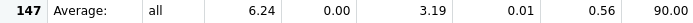
\includegraphics[width=\linewidth]{img/SC1_CPUAVG.png}
	\caption{Gemiddeld CPU gebruik (100 - Laatste Kolom).}
	\label{fig:SC1_CPUAVG}
\end{figure}
\begin{figure}[h]
	\centering
	\begin{minted}{bash} 
> summary(ram)
RAM       
Min.   :89.33  
1st Qu.:89.75  
Median :90.11  
Mean   :90.13  
3rd Qu.:90.39  
Max.   :91.25
	\end{minted}
	\caption{Gemiddeld RAM gebruik}
	\label{SC1_RAMAVG}
\end{figure}

Ten tweede zullen de gegevens in verband met de stabiliteit van het systeem bekeken worden. In figuur \ref{fig:SC1_CPUBox} en \ref{fig:SC1_RAMBox} zijn de boxplots voor zowel het CPU als RAM gebruik te zien. We kunnen zien dat bij het CPU gebruik er maar 3 \textit{outliers} zijn en bij het RAM gebruik zijn er zelf geen \textit{outliers}. Dit wijst erop dat het RAM gebruik zeer stabiel blijft. 

%\begin{figure}[ht]
%	\centering
%	\begin{minipage}[b]{0.75\linewidth}
%		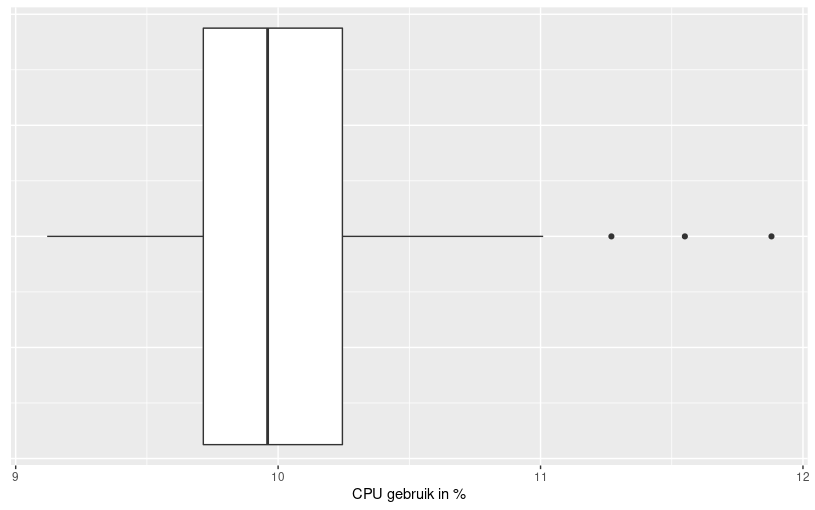
\includegraphics[width=\linewidth]{img/SC1_CPUBox.png}
%		\caption{Boxplot van het CPU gebruik in Scenario 1}
%		\label{fig:SC1_CPUBox}
%	\end{minipage}
%	\quad
%	\begin{minipage}[b]{0.75\linewidth}
%		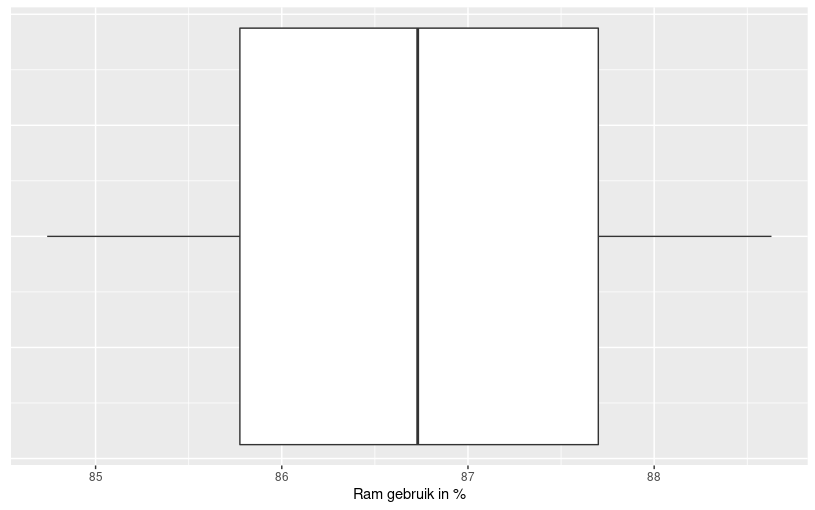
\includegraphics[width=\linewidth]{img/SC1_RAMBox.png}
%		\caption{Boxplot van het RAM gebruik in Scenario 1}
%		\label{fig:SC1_RAMBox}
%	\end{minipage}
%\end{figure}
%
\begin{figure}[h]
	\centering
	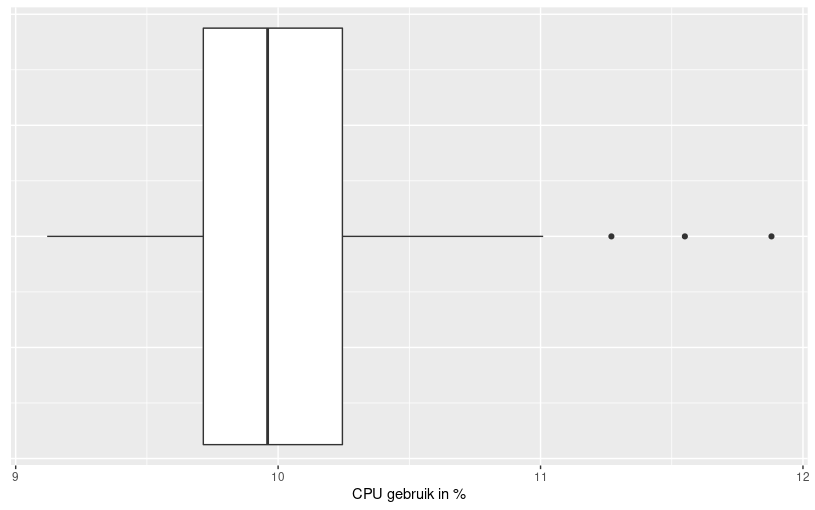
\includegraphics[width=0.75\linewidth]{img/SC1_CPUBox.png}
	\caption{Boxplot van het CPU gebruik in Scenario 1}
	\label{fig:SC1_CPUBox}
\end{figure}

\begin{figure}[h]
	\centering
	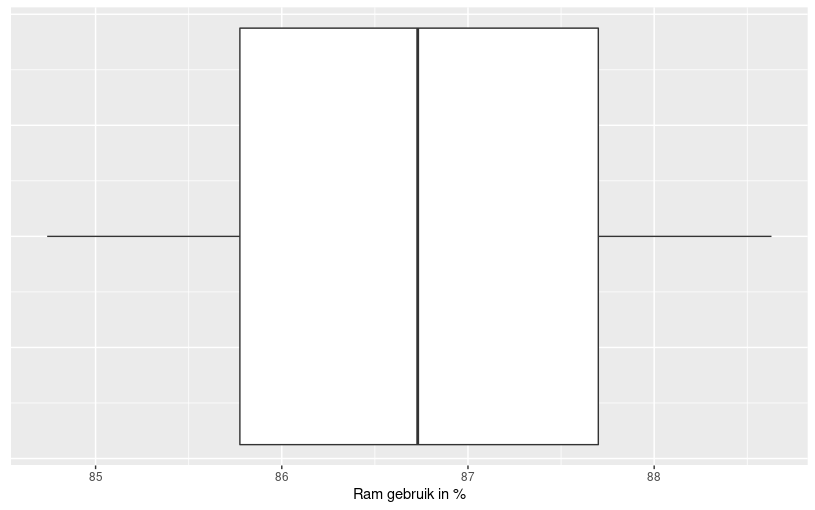
\includegraphics[width=0.75\linewidth]{img/SC1_RAMBox.png}
	\caption{Boxplot van het RAM gebruik in Scenario 1}
	\label{fig:SC1_RAMBox}
\end{figure}

Als derde criteria worden de gegevens van het algemene CPU en RAM gebruik bekeken. Deze worden gevisualiseerd aan de hand van een lijngrafiek. Het resultaat van scenario 1 is te zien in figuur \ref{fig:SC1_CPUGraph} en \ref{fig:SC1_RAMGraph}.

\begin{figure}[h]
	\centering
	\begin{minipage}[b]{0.45\linewidth}
			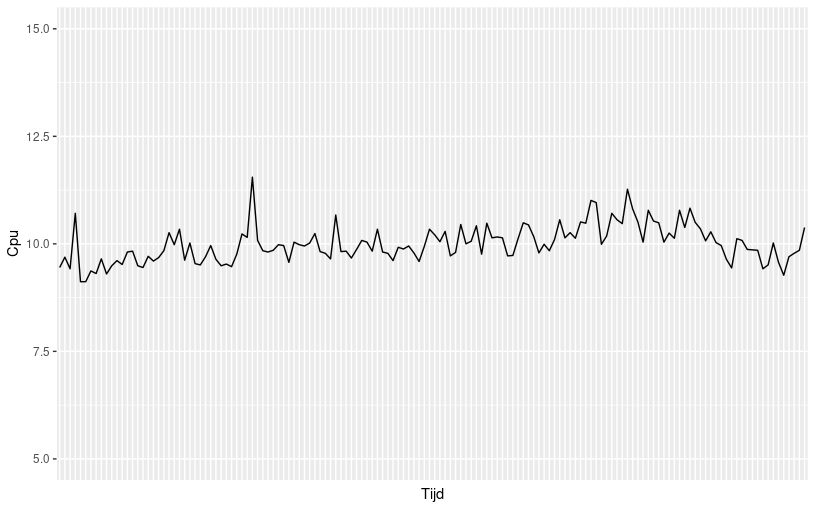
\includegraphics[width=\linewidth]{img/SC1_CPUGraph.png}
		\caption{Lijngrafiek van het CPU gebruik in Scenario 1.}
		\label{fig:SC1_CPUGraph}
	\end{minipage}
	\quad
	\begin{minipage}[b]{0.45\linewidth}
		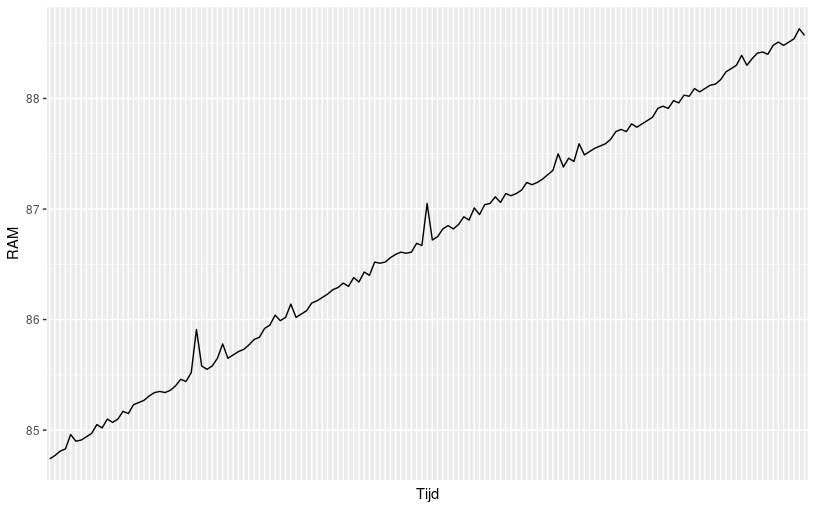
\includegraphics[width=\linewidth]{img/SC1_RAMGraph.png}
		\caption{Lijngrafiek van het RAM gebruik in Scenario 1.}
		\label{fig:SC1_RAMGraph}
	\end{minipage}
\end{figure}


Het laatste criteria is de opstarttijd van de node. Deze kan men simpelweg vinden aan de hand van het \verb|systemd-analyze| commando. De uitvoer van dit commando is te zien in figuur \ref{SC1_StartTime}.

\begin{figure}[h]
	\centering
	\begin{minted}{bash} 
$ systemd-analyze
Startup finished in 6.121s (kernel) + 3.296s (userspace) = 9.418s
	\end{minted}
	\caption{Opstarttijd van de Node in Scenario 1}
	\label{SC1_StartTime}
\end{figure}

%1e is gemiddelde
%2e is boxplot
%3e is Graph
%4e is opstarttijd

\clearpage
\subsection{Scenario 2}
% Node 45.79.249.208 wordt gebruikt
Als eerste zal het gemiddelde gebruik van zowel de CPU als het RAM geheugen verzameld worden. Voor de CPU is dit 10.15\% zoals te zien in figuur \ref{fig:SC2_CPUAVG}. Het gemiddelde RAM gebruik is af te lezen wanneer we de code uit figuur \ref{RAMAVG} uitvoeren op de dataset. De uitvoer hiervan is 90.75\%, zoals in figuur \ref{SC2_RAMAVG} te zien is.
\begin{figure}[h]
	\centering
	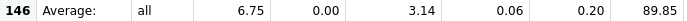
\includegraphics[width=\linewidth]{img/SC2_CPUAVG.png}
	\caption{Gemiddeld CPU gebruik (100 - Laatste Kolom).}
	\label{fig:SC2_CPUAVG}
\end{figure}
\begin{figure}[h]
	\centering
	\begin{minted}{bash} 
> summary(ram)
RAM       
Min.   :90.21  
1st Qu.:90.60  
Median :90.74  
Mean   :90.75  
3rd Qu.:90.91  
Max.   :91.27  
	\end{minted}
	\caption{Gemiddeld RAM gebruik in Scenario 2}
	\label{SC2_RAMAVG}
\end{figure}

Ten tweede zullen de gegevens in verband met de stabiliteit van het systeem bekeken worden. In figuur \ref{fig:SC2_CPUBox} en \ref{fig:SC2_RAMBox} zijn de boxplots voor zowel het CPU als RAM gebruik te zien. We kunnen zien dat bij het CPU gebruik er 4 \textit{outliers} zijn en bij het RAM gebruik zijn er zelf geen \textit{outliers}. 

%\begin{figure}[ht]
%	\centering
%	\begin{minipage}[b]{0.75\linewidth}
%		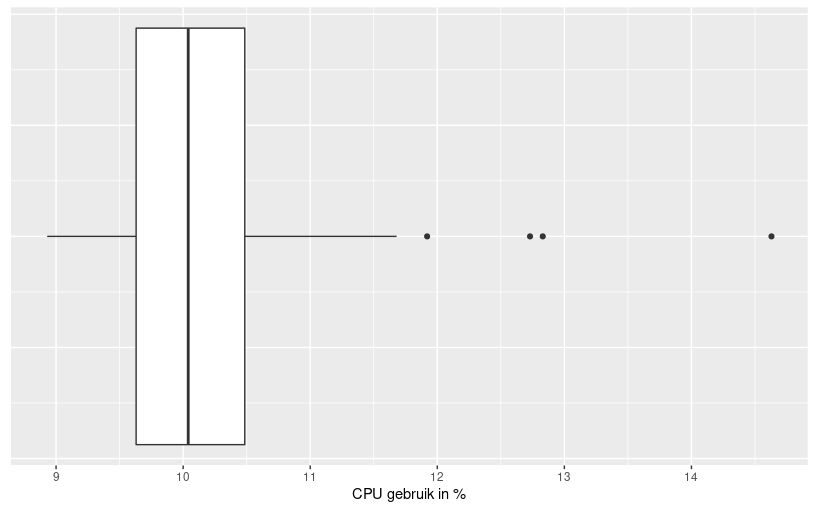
\includegraphics[width=\linewidth]{img/SC2_CPUBox.png}
%		\caption{Boxplot van het CPU gebruik in Scenario 2.}
%		\label{fig:SC2_CPUBox}
%	\end{minipage}
%	\quad
%	\begin{minipage}[b]{0.75\linewidth}
%		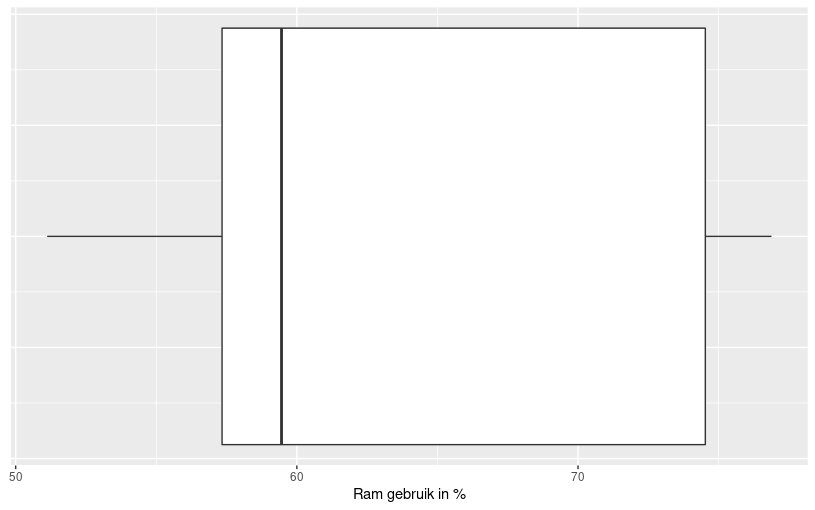
\includegraphics[width=\linewidth]{img/SC2_RAMBox.png}
%		\caption{Boxplot van het RAM gebruik in Scenario 2.}
%		\label{fig:SC2_RAMBox}
%	\end{minipage}
%\end{figure}
%
\begin{figure}[h]
	\centering
	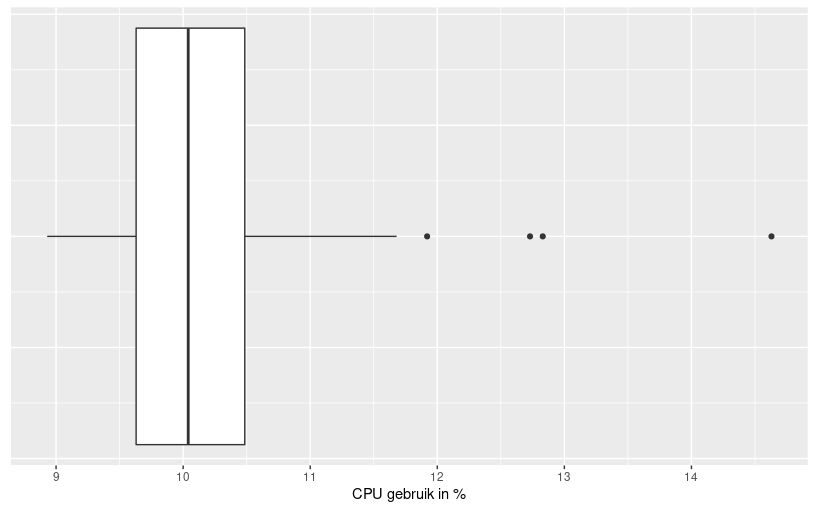
\includegraphics[width=0.75\linewidth]{img/SC2_CPUBox.png}
	\caption{Boxplot van het CPU gebruik in Scenario 2}
	\label{fig:SC2_CPUBox}
\end{figure}

\begin{figure}[h]
	\centering
	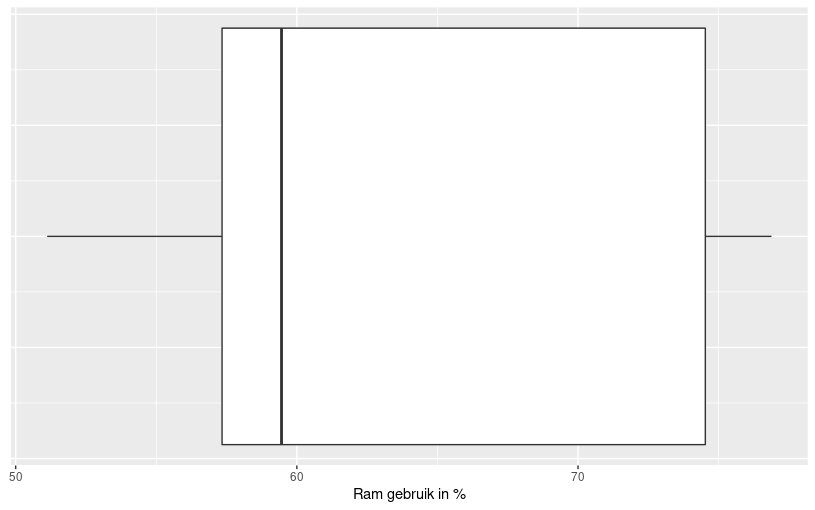
\includegraphics[width=0.75\linewidth]{img/SC2_RAMBox.png}
	\caption{Boxplot van het RAM gebruik in Scenario 2}
	\label{fig:SC2_RAMBox}
\end{figure}


Als derde criteria worden de gegevens van het algemene CPU en RAM gebruik bekeken. Deze worden gevisualiseerd aan de hand van een lijngrafiek. Het resultaat van scenario 1 is te zien in figuur \ref{fig:SC2_CPUGraph} en \ref{fig:SC2_RAMGraph}. 
\begin{figure}[h]
	\centering
	\begin{minipage}[h]{0.45\linewidth}
		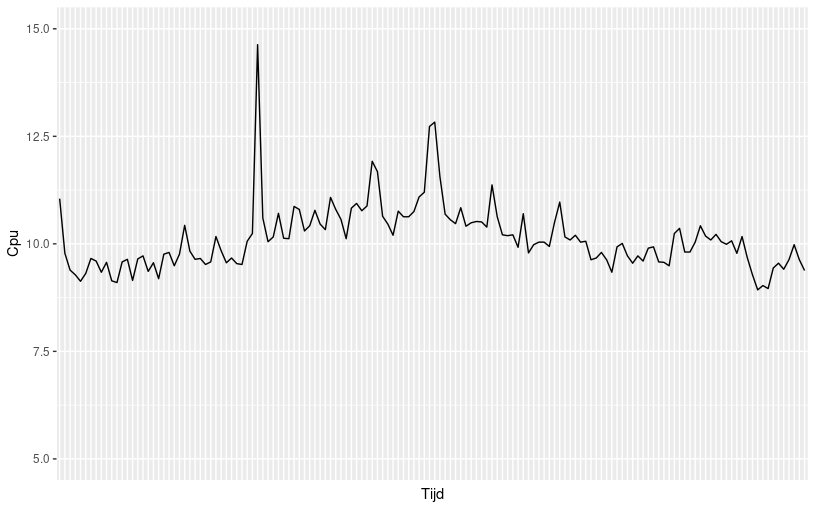
\includegraphics[width=\linewidth]{img/SC2_CPUGraph.png}
		\caption{Lijngrafiek van het CPU gebruik in Scenario 2.}
		\label{fig:SC2_CPUGraph}
	\end{minipage}
	\quad
	\begin{minipage}[h]{0.45\linewidth}
		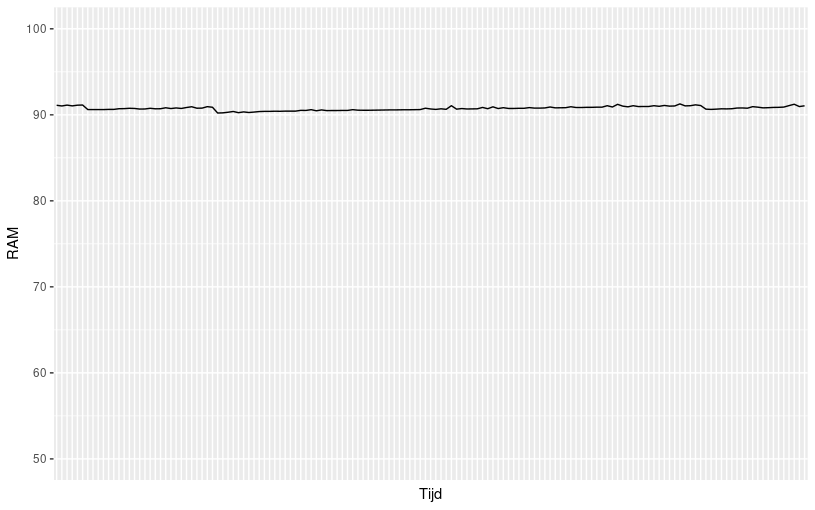
\includegraphics[width=\linewidth]{img/SC2_RAMGraph.png}
		\caption{Lijngrafiek van het RAM gebruik in Scenario 2.}
		\label{fig:SC2_RAMGraph}
	\end{minipage}
\end{figure}

%\begin{figure}[h]
%	\centering
%	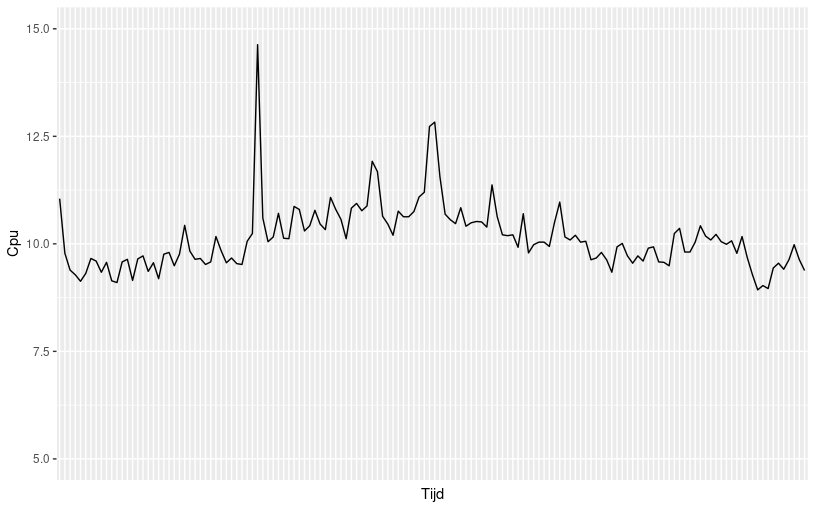
\includegraphics[width=0.75\linewidth]{img/SC2_CPUGraph.png}
%	\caption{Boxplot van het CPU gebruik in Scenario 2}
%	\label{fig:SC2_CPUGraph}
%\end{figure}
%
%\begin{figure}[h]
%	\centering
%	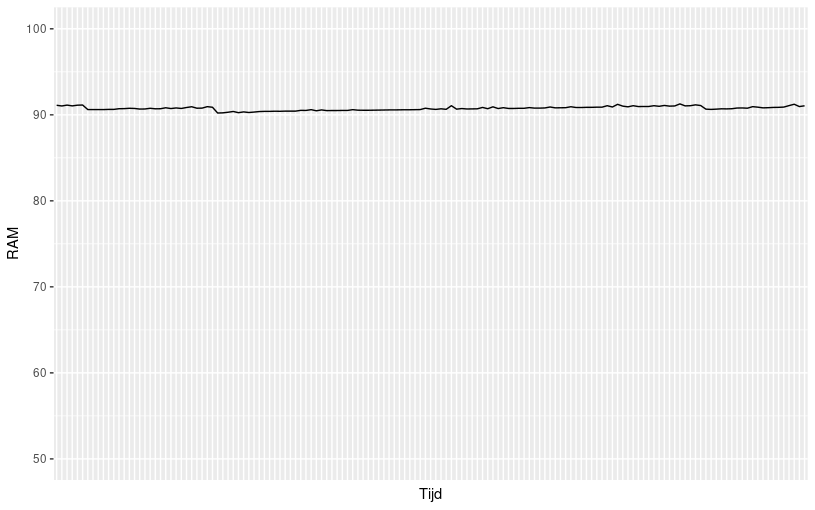
\includegraphics[width=0.75\linewidth]{img/SC2_RAMGraph.png}
%	\caption{Boxplot van het RAM gebruik in Scenario 2}
%	\label{fig:SC2_RAMGraph}
%\end{figure}


Het laatste criteria is de opstarttijd van de node. Deze kan men simpelweg vinden aan de hand van het \verb|systemd-analyze| commando. De uitvoer van dit commando is te zien in figuur \ref{SC2_StartTime}.

\begin{figure}[h]
	\centering
	\begin{minted}{bash} 
$ systemd-analyze
Startup finished in 6.246s (kernel) + 2.997s (userspace) = 9.243s
	\end{minted}
	\caption{Opstarttijd van de Node in Scenario 2}
	\label{SC2_StartTime}
\end{figure}

\clearpage
\subsection{Scenario 3}
% node 172.105.86.96 wordt gebruikt
%Data verzamelen over kube-bench door ./repeat.sh uit te voeren zodat dit zichtbaar is in de sar logs
%Kubebench even laten runnen zodat er een spike komt
%
%Kube hunter op de drie manieren uitvoeren op deze cluster 
%	op een node installeren
%	een node van de andere cluster scannen
%	een bad pod erin smijten

Als eerste zal het gemiddelde gebruik van zowel de CPU als het RAM geheugen verzameld worden. Voor de CPU is dit 12.3\% zoals te zien in figuur \ref{fig:SC3_CPUAVG}. Het gemiddelde RAM gebruik is af te lezen wanneer we de code uit figuur \ref{RAMAVG} uitvoeren op de dataset. De uitvoer hiervan is 90.13\%, zoals in figuur \ref{SC3_RAMAVG} te zien is.
\begin{figure}[h]
	\centering
	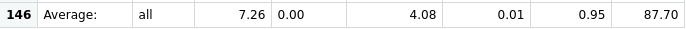
\includegraphics[width=\linewidth]{img/SC3_CPUAVG.png}
	\caption{Gemiddeld CPU gebruik (100 - Laatste Kolom).}
	\label{fig:SC3_CPUAVG}
\end{figure}
\begin{figure}[h]
	\centering
	\begin{minted}{bash} 
> summary(ram)
RAM       
Min.   :89.33  
1st Qu.:89.75  
Median :90.11  
Mean   :90.13  
3rd Qu.:90.39  
Max.   :91.25    
	\end{minted}
	\caption{Gemiddeld RAM gebruik}
	\label{SC3_RAMAVG}
\end{figure}

Ten tweede zullen de gegevens in verband met de stabiliteit van het systeem bekeken worden. In figuur \ref{fig:SC3_CPUBox} en \ref{fig:SC3_RAMBox} zijn de boxplots voor zowel het CPU als RAM gebruik te zien. Bij het CPU gebruik zien we 11 outliers en bij het RAM gebruik zijn er geen outliers. Dit wijst er op dat het CPU gebruik minder stabiel blijkt te zijn in vergelijking met de vorige Scenario's.

%\begin{figure}[ht]
%	\centering
%	\begin{minipage}[b]{0.75\linewidth}
%		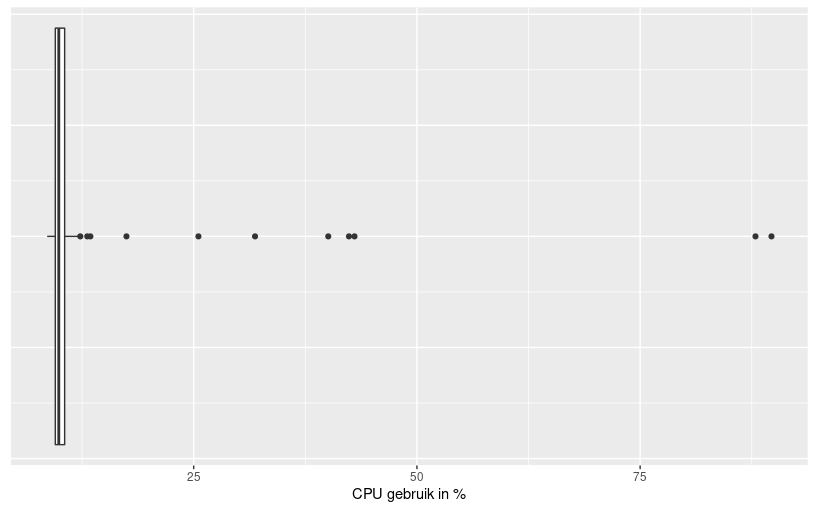
\includegraphics[width=\linewidth]{img/SC3_CPUBox.png}
%		\caption{Boxplot van het CPU gebruik in Scenario 3}
%		\label{fig:SC3_CPUBox}
%	\end{minipage}
%	\quad
%	\begin{minipage}[b]{0.75\linewidth}
%		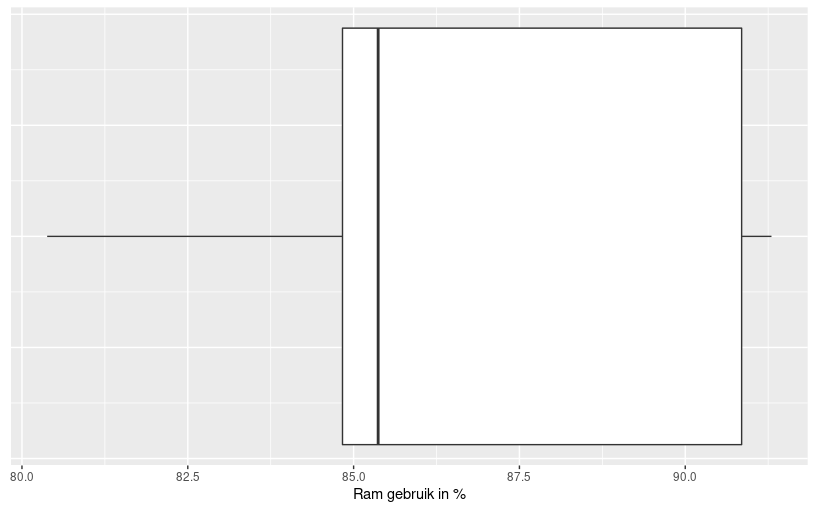
\includegraphics[width=\linewidth]{img/SC3_RAMBox.png}
%		\caption{Boxplot van het RAM gebruik in Scenario 3}
%		\label{fig:SC3_RAMBox}
%	\end{minipage}
%\end{figure}


\begin{figure}[h]
	\centering
	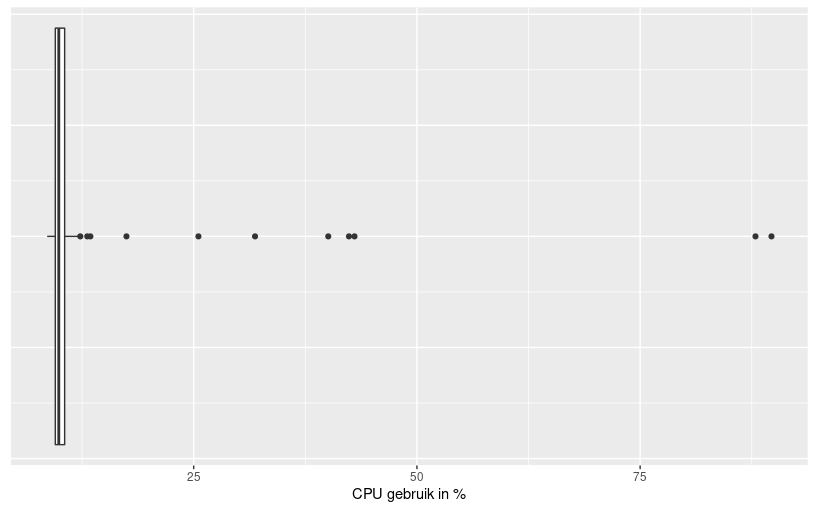
\includegraphics[width=0.75\linewidth]{img/SC3_CPUBox.png}
	\caption{Boxplot van het CPU gebruik in Scenario 3}
	\label{fig:SC3_CPUBox}
\end{figure}

\begin{figure}[h]
	\centering
	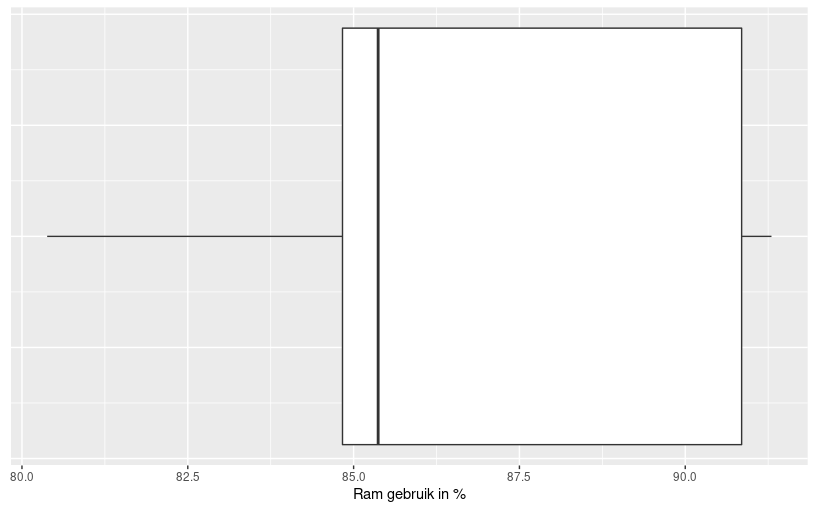
\includegraphics[width=0.75\linewidth]{img/SC3_RAMBox.png}
	\caption{Boxplot van het RAM gebruik in Scenario 3}
	\label{fig:SC3_RAMBox}
\end{figure}


Als derde criteria worden de gegevens van het algemene CPU en RAM gebruik bekeken. Deze worden gevisualiseerd aan de hand van een lijngrafiek. Het resultaat van scenario 1 is te zien in figuur \ref{fig:SC3_CPUGraph} en \ref{fig:SC3_RAMGraph}. De eerste piek in CPU gebruik is te wijten aan het gebruik van Kube-bench terwijl de tweede en derde piek zijn veroorzaakt door het gebruik van Kube-hunter.
\begin{figure}[h]
	\centering
	\begin{minipage}[h]{0.45\linewidth}
		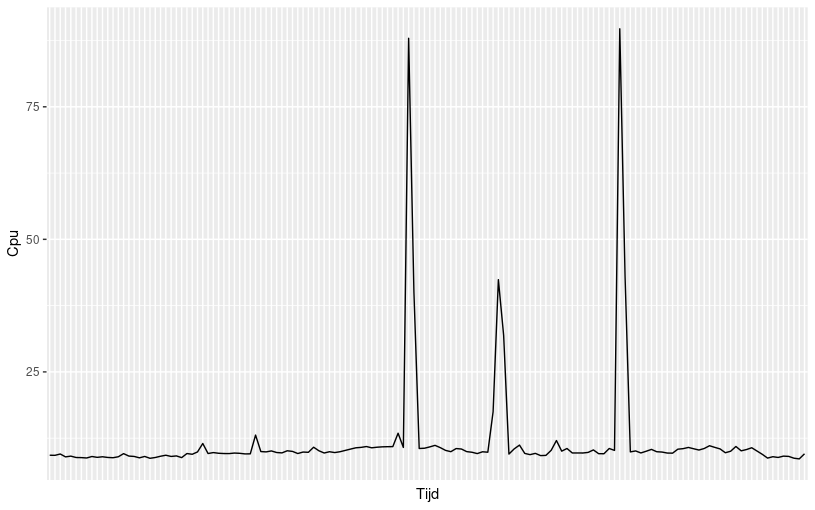
\includegraphics[width=\linewidth]{img/SC3_CPUGraph.png}
		\caption{Lijngrafiek van het CPU gebruik in Scenario 3.}
		\label{fig:SC3_CPUGraph}
	\end{minipage}
	\quad
	\begin{minipage}[h]{0.45\linewidth}
		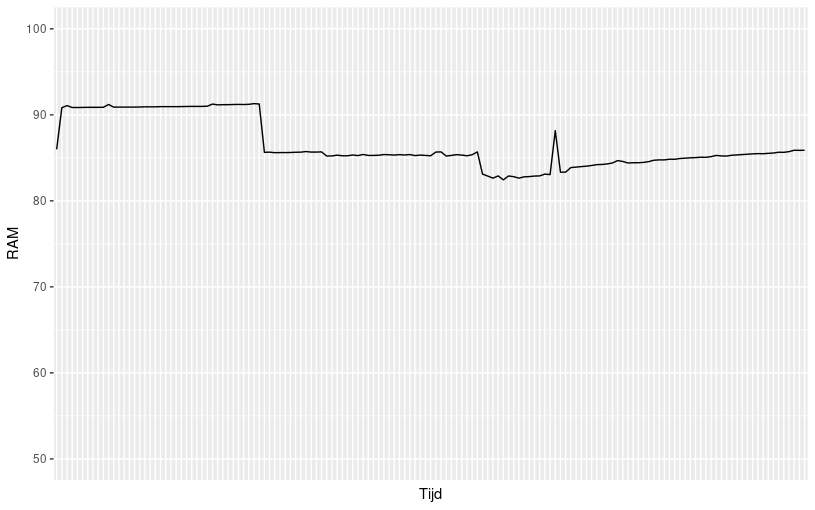
\includegraphics[width=\linewidth]{img/SC3_RAMGraph.png}
		\caption{Lijngrafiek van het RAM gebruik in Scenario 3.}
		\label{fig:SC3_RAMGraph}
	\end{minipage}
\end{figure}


Het laatste criteria is de opstarttijd van de node. Deze kan men simpelweg vinden aan de hand van het \verb|systemd-analyze| commando. De uitvoer van dit commando is te zien in figuur \ref{SC3_StartTime}.

\begin{figure}[h]
	\centering
	\begin{minted}{bash} 
$ systemd-analyze
Startup finished in 6.153s (kernel) + 5.180s (userspace) = 11.334s
	\end{minted}
	\caption{Opstarttijd van de Node in Scenario 3}
	\label{SC3_StartTime}
\end{figure}

\clearpage
\subsection{Vergelijken van de data}
Nu alle gegevens verzameld en verwerkt zijn kunnen we deze met elkaar gaan vergelijken. Als eerste zal het gemiddeld \textit{resource} gebruik van de verschillende scenario's besproken worden. Tabel \ref{tab:AVGResource} geeft een overzicht van de data. In deze tabel is duidelijk te zien dat zowel de \textit{best practices} als de beveiligings-tools een invloed hebben gehad op het CPU gebruik. De hoeveelheid RAM die gebruikt werd is daarentegen hetzelfde gebleven bij zowel Scenario één als drie. Deze is in scenario twee zelfs gezakt. Ook al werden in scenario drie de tools maar sporadisch gebruikt, toch hebben deze een aanzienlijke impact op het gemiddeld \textit{resource} gebruik van de cluster gehad. 
\begin{table}[h]
	\centering
	\begin{tabular}{lccc}
		Gemiddeld resource gebruik & Scenario1 & Scenario2 & Scenario3 \\ \hline
		CPU                        & 10        & 10.15        & 12.3      \\ \hline
		Ram                        & 90.13     & 90.75        & 90.13    
	\end{tabular}
	\caption{Gemiddeld resource gebruik van de scenario's}
	\label{tab:AVGResource}
\end{table}

Het tweede criteria dat onderzocht werd is de stabiliteit van de cluster, dit door het aantal \textit{outliers} te tellen. In tabel \ref{tab:Outliers} is te zien hoeveel \textit{outliers} er per scenario werden gedetecteerd. Geen enkel scenario had effect op de stabiliteit van het RAM gebruik maar het CPU gebruik werd wel iets instabieler in scenario drie. Deze grote hoeveelheid \textit{outliers} is te wijten aan het feit dat de beveiligings-tools niet constant in gebruik zijn. De \textit{outliers} komen hier dus overeen met de momenten waarop de tools actief werden gebruikt. Hieruit is te concluderen dat \textit{best practices} een kleine (praktisch verwaarloosbare) impact hebben op de stabiliteit. Alsook dat beveiligings-tools een tijdelijke maar toch aanzienlijk effect hebben op de data.
%
\begin{table}[h]
	\centering
	\begin{tabular}{lccc}
		Aantal outliers & Scenario1 & Scenario2 & Scenario3 \\ \hline
		CPU             & 3         & 4         & 11        \\ \hline
		Ram             & 0         & 0         & 0        
	\end{tabular}
	\caption{Aantal outliers van de scenario's}
	\label{tab:Outliers}
\end{table}

Het laatste criteria dat werd onderzocht is de opstart tijd van een node in de cluster. Tabel \ref{tab:BootTime} toont de hoeveelheid seconden de node in elk scenario nodig had om op te starten. Deze tabel maakt duidelijk dat \textit{best practices} geen (of in dit geval een positief) effect hebben op de opstarttijd van een cluster. De beveiligings-tools aan de andere kant zorgde er voor dat de node twee seconden trager opstarten. 

\begin{table}[h]
	\centering
	\begin{tabular}{lccc}
		& Scenario1 & Scenario2 & Scenario3 \\ \hline
		Opstarttijd & 9.418     & 9.243     & 11.334   
	\end{tabular}
	\caption{Tijd die de Node nodig had om op te starten}
	\label{tab:BootTime}
\end{table}


